\documentclass{deimj}
\usepackage[dvipdfmx]{graphicx}
\usepackage[ipaex]{pxchfon}
\usepackage[hyphens]{url}
\usepackage{tabularx}
\usepackage{multirow}

% 印刷位置調整 %
% 必要に応じて値を変更してください.
\hoffset -10mm % <-- 左に 10mm 移動
\voffset -10mm % <-- 上に 10mm 移動

\newcommand{\AmSLaTeX}{%
$\mathcal A$\lower.4ex\hbox{$\!\mathcal M\!$}$\mathcal S$-\LaTeX}
\newcommand{\PS}{{\scshape Post\-Script}}
\def\BibTeX{{\rmfamily B\kern-.05em{\scshape i\kern-.025em b}\kern-.08em
T\kern-.1667em\lower.7ex\hbox{E}\kern-.125em X}}

\papernumber{DEIM Forum 2019 XX-Y}

% \jtitle{未訪問エリアの理解支援のための既訪問スポットに基づく類推情報提示手法}
\jtitle{ユーザの既訪問スポットの位置づけに基づく未訪問スポットの説明手法}
%\jsubtitle{サブタイトル} <- サブタイトルを付けたいときはこの行の先頭の % を取る
\authorlist{%
 \authorentry[em18011@ns.kogakuin.ac.jp]{潘 健太}{KENTA HAN}{UnivN}
 \authorentry[kitayama@cc.kogakuin.ac.jp]{北山 大輔}{DAISUGE KITAYAMA}{UnivN}
 }

\affiliate[UnivN]{工学院大学大学院工学研究科情報学専攻\hskip1zw
  〒163--8677 西新宿1-24-2}
 {School of Engineering,Kogakuin University\\
  1--24--2,Nisisinjyuku,Tokyo,163--8677 Japan}

\begin{document}
\pagestyle{empty}
\begin{jabstract}
近年,観光スポットを決める時にWeb上の観光情報を活用して計画を立てることが多くなっている.
しかし,ユーザが多くのエリアから訪問したいエリアを決めた上で,さらに自分のイメージに合う観光スポットを探すのは膨大な時間と労力を必要とする.
また,ユーザが未訪問スポットに対して期待と不安を感じる場合がある.
%以前に経験した事柄を,現在直面している事柄あるいは問題にあてはめることを類推と呼ぶ.
本研究では,ユーザの未知なスポットに対する理解を支援するためには,既に訪問したことがある観光スポットの特徴を未訪問スポットにあてはめて理解を支援する説明手法を提案する.
観光スポット自身の特徴を重視するため,各観光スポットの特徴抽出に,ユーザが入力した観光スポットのすべてのレビュー,対象エリアの観光スポットのすべてのレビューを使用する.
また,プロトタイプシステムを構築し,既訪問スポットと未訪問スポットとの説明情報の効果を検証する評価実験を行う.
\end{jabstract}

\begin{jkeyword}
% 観光スポット,理解支援,レビュー,コサイン類似度,TFIDF,調和平均
観光スポット,理解支援,レビュー,分散表現
\end{jkeyword}
\maketitle


%%%%%%%%%%%%%%%%%%%%%%%%%%%%%%%%%%%%%%%%%%
%%%%%%%%%%%%%%%%%%%%%%%%%%%%%%%%%%%%%%%%%%
\section{はじめに}
\label{sec:はじめに}
%%%%%%%%%%%%%%%%%%%%%%%%%%%%%%%%%%%%%%%%%%
%%%%%%%%%%%%%%%%%%%%%%%%%%%%%%%%%%%%%%%%%%
旅行先を決定する時,旅行者は観光スポット検索サイトや観光情報に関連する書籍を見て観光スポットを選び,旅行計画を立てる.
しかし,ユーザにとって訪問したいエリアを決定した後,さらにエリア内に数多く存在する観光スポットから,自身のイメージから外れない観光スポットを見つけることは容易ではない.
行きたい観光スポットが決まっていない場合ではランキングやおすすめ情報を見て観光スポットを決めることが多くなると考えられる.
この時,ユーザが選択した観光スポットに対するイメージが曖昧になるため不安を感じる場合がある.

近年,観光業とソーシャルネットワーキングサービスの発展スピードが加速しており,体験した観光スポットに対するレビューを観光スポット検索サイトに投稿しているユーザが増加している.
さまざまな観光スポットを効果的に理解するためには,既存の情報をもとにして,未知な情報と既知な情報との対応関係を考えることが不可欠となる.
この考え方は,以前に経験した事柄(ベースと呼ぶ)を,現在直面している事柄あるいは問題(ターゲットと呼ぶ)にあてはめる類推に相当する.
たとえば,金沢の「にし茶屋街」という未知なスポットに対して既訪問の京都の「花見小路」と似ていると説明するとイメージの理解がしやすくすることがある.

本研究では,ユーザの未訪問スポットに対する理解を支援するため,既に訪問したことがある観光スポットの特徴を未訪問スポットにあてはめて理解を支援する説明手法を提案する.
具体的には,ユーザが入力した既訪問スポットと未訪問エリアから,レビュを用いて既訪問スポット内の各スポットの独特な特徴と未訪問エリア内の各スポットの独特な特徴を抽出し,比較を行って説明情報を提示する.
このプロトタイプシステムにより,ユーザが未訪問スポットに対する理解の支援を目指す.図\ref{fig:photo_image}は提案手法の概念図である.

本論文の構成は下記のとおりである.
2章では関連研究について述べる.
3章では提案手法の概要について述べる.
4章では構築したプロトタイプシステムの効果を検証する評価実験と考察について述べる.
最後に5章ではまとめと今後の課題について述べる.
%3節,4節の間は予備実験を追加する可能性がある%

\begin{figure}[t]
  \begin{center}
    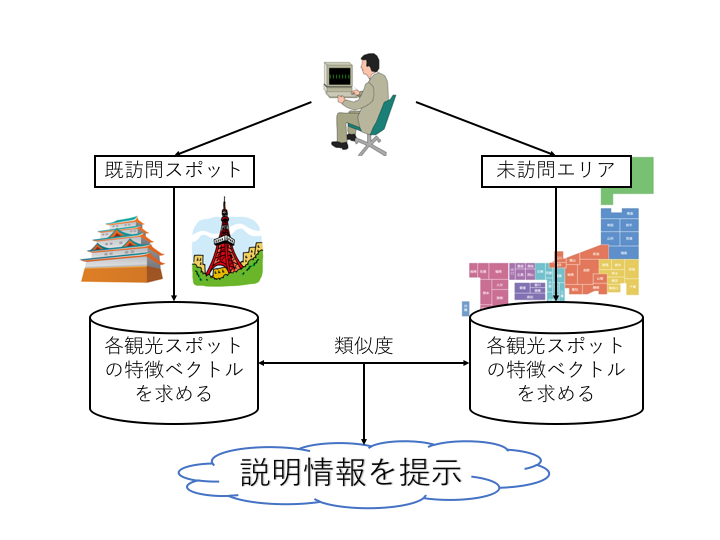
\includegraphics[clip,width=7.0cm]{picture/Photo_Image_jap.png}
    \caption{ユーザの既訪問スポットの位置づけに基づく未訪問スポット(エリア)の説明手法}
    \label{fig:photo_image}
   \end{center}
\end{figure}


%%%%%%%%%%%%%%%%%%%%%%%%%%%%%%%%%%%%%%%%%%
%%%%%%%%%%%%%%%%%%%%%%%%%%%%%%%%%%%%%%%%%%
\section{関連研究}
\label{sec:関連研究}
%%%%%%%%%%%%%%%%%%%%%%%%%%%%%%%%%%%%%%%%%%
%%%%%%%%%%%%%%%%%%%%%%%%%%%%%%%%%%%%%%%%%%
% クチコミを使用した地理情報の検索および推薦に関する研究は数多く行われている.
% 廣嶋ら\cite{Codd01}は,地理情報検索の際のクエリ入力支援として,提示する特徴語の抽出手法について研究を行った.
% この手法では,各ブログ記事から特徴語候補の抽出および地点の特定を行った.
% 具体的には,特徴語の候補をWikipediaの見出し語に限定し,ポアソン確率を用いて特徴語抽出を行った.
%
% 観光地検索するとき,松本ら\cite{Codd02}はクチコミから特徴語を抽出して利用する研究を行なった.
% 抽出対象を任意の名詞として,4種類の手法,TFIDF,ATF(Average Term Frequency),ポアソン確率,エントロピーのうちどの手法が特徴語抽出に適しているのか検討を行なった.
% また,抽出した特徴語を利用した検索支援システムを試作し,実験を通して特徴語提示の効果を検証した.
%
% 上原ら\cite{Codd03}はWebから観光情報を抽出し,複数の特徴ベクトルから観光地間の類似性を評価することで,観光地を推薦するシステムを提案した.
% 観光地の特徴ベクトルは,知恵袋・ブログ上での共起キーワードと時系列分布,知恵袋上でのカテゴリ構造,観光地周辺施設,地図画像から生成した.
% これらの特徴ベクトルから観光地間の類似度の測定を行い,類似度の高い観光地を推薦した.
%
% 野守ら\cite{Codd04}は日本全国の観光地のクチコミデータを用いて,観光客が話題にする観光テーマを確率的に抽出し,そのテーマを軸として各観光地の特徴を定量的に評価した.また,クチコミのテキストデータにテキストマイニングを実行して表現を抽出し,観光地ごとにその表現の出現頻度を集計したクロス集計表にPLSAを実行することで,観光客のクチコミだけに基づいた観光テーマの抽出と観光地の特徴分析を行なった.
%
% 類推に関する研究の数多くは,ベースとなる物語とターゲットとなる問題が与えられ,物語の特徴を問題の特徴にマッピングして問題を解決するものである\cite{Codd05}.
% 石田ら\cite{Codd06}は新知識を理解するための類推能力の育成についての研究を行った.
% 具体名詞を明確な事物,抽象名詞を不明確な事物とし,明確な事物をターゲットとして扱う.
% 類推による新知識の理解の枠組みを実装したシステムを利用することで,類推プロセスの理解と繰り返しによる練習を促し,類推能力を育成できるのかについて検証を行った.
% 砂山ら\cite{Codd07}は自身が知っている知識を,その知識を知らない他人に伝える際に,類推を用いて分かりやすく説明するスキルの獲得を支援するシステムを提案した.
% 評価実験により,システムを用いた被験者が,分かりやすい説明を行える能力を身につけられる可能性を確認した.
% 中村ら\cite{Codd08}は新たな概念を創造しようとするとき,本質的な役割を果たす高次認知機能として類推に着目して研究を行った.構造の類似性には3種類あり,特徴の共有数で決まる「対象レベルの類似性」,ベースに存在する関係とターゲットに存在する関係の共有度に基づく「関係レベルの類似性」,および題の解法あるいは目標レベルでの類似性である「プラグマティックな類似性」とがある\cite{Codd09}.
%
% 従来のレビューを利用する手法では,クチコミを分析して,対象目標の検索をしやすくための研究が多い.
% また,類推技術は学習支援でよくて使われている.
% 本研究,提案する未訪問エリアの理解支援のための既訪問スポットに基づく類推情報提示手法は,既訪問スポットと未訪問エリアのレビューを使い,未知ターゲットに対する理解を支援するため,類推の質を明示的扱う.
% そのため,構造の類似性「関係レベルの類似性」に近いと考えられる.

ユーザの体験履歴を利用した検索や推薦システムに関する研究が数多く発表されている.
倉島ら\cite{Codd07}は,Flickrに投稿された写真のジオタグ情報を人々の旅行履歴として利用した旅行ルート推薦手法を提案した.
この手法では,ユーザの現在地から行きやすい場所とユーザの興味に合致した場所に移動しやすいと仮定し,行動モデルを生成している.
ユーザのジオタグ付き写真集合は,時間情報でソートすると個人の旅行履歴とみなすことができると考え,ジオタグ情報を利用してユーザの行動モデルを生成している.
北村らは\cite{Codd08},一般的な物体認識を用いて,過去の個人旅行写真から旅行計画のユーザの嗜好を推定することに基づいて観光地を推薦する方法を提案した.
物体認識システムを用いて,写真で撮った被写体情報のキーワードを取得し,グラフ視覚化技術によってキーワードの共起を表現した.
また,グラフの視覚化技術に基づいて旅行写真付きのグラフを視覚化するユーザインターフェイスを紹介した.
Chengらは\cite{Codd09},自由に利用できるコミュニティ寄稿の写真を活用して,パーソナライズされた旅行のおすすめに焦点を当て,特定のユーザープロファイルまたは属性を考慮し,パーソナライズされた旅行の推奨を行うことを提案した.

類推は創造的思考に貢献すると指摘されてた\cite{Codd01}.
既知の知識(ベースと呼ぶ)から概念(ターゲットと呼ぶ)を獲得するときに類推思考が働くとされる\cite{Codd02}.
類推に関する研究の多くは,ベースとなる学習データとターゲットとなる問題が与えられ,物事の特徴を問題の特徴にマッピングして問題を解決するもの\cite{Codd03}である.
Gickらは,不確定な問題の解を見つけるためのガイドとして,異種ドメイン間の類推の使用を調査するように設計した.
学習データの与え方や機能について研究したもの\cite{Codd04}や,認知的な熟達度に応じて問題を解決するかどうかを明らかにしたもの\cite{Codd05}がある.
これらを含む従来研究の多くにおいては,類推に用いるベースとターゲットを与えたうえで,一定の手順に従って問題解決を行っている.また,構造の類似性には3種類あり,特徴の共有数で決まる「対象レベルの類似性」,ベースに存在する関係とターゲットに存在する関係の共有度に基づく「関係レベルの類似性」,および題の解法あるいは目標レベルでの類似性である「プラグマティックな類似性」とがある.

従来のユーザの体験履歴を利用する手法では,履歴写真のジオタグ情報を分析し,ユーザの嗜好とする研究が多く行われている.
また,類推技術に関して学習支援でよくて使われている.
本研究では,既訪問スポットと未訪問スポットのレビューを使って,ユーザ既訪問スポット集合と未訪問スポット集合のそれぞれ集合の各スポットの相対的な特徴を求め,関連付けることによって,スポットに対する理解を支援するため説明情報を提示することができる.また,本研究では,類推の質を明示的扱うため,構造の類似性「関係レベルの類似性」に近いと考えられる.

%%%%%%%%%%%%%%%%%%%%%%%%%%%%%%%%%%%%%%%%%%
%%%%%%%%%%%%%%%%%%%%%%%%%%%%%%%%%%%%%%%%%%
\section{未訪問スポットの説明手法}
\label{sec:未訪問スポットの説明手法}
%%%%%%%%%%%%%%%%%%%%%%%%%%%%%%%%%%%%%%%%%%
%%%%%%%%%%%%%%%%%%%%%%%%%%%%%%%%%%%%%%%%%%
我々は,ユーザの既訪問スポットの位置づけに基づく未訪問スポットの説明手法を提案する.
具体的にはまず,ユーザが既訪問の複数個の観光スポットと訪問したい観光スポットエリア情報を入力する.
既訪問スポットレビューベクトルを使って既訪問スポット毎の特徴ベクトルを求める.
未訪問スポットも同様にエリア内の各スポットの特徴ベクトルを求める.
次に,既訪問スポットレビューベクトルと未訪問スポットレビューベクトルの差分特徴に類似する特徴を持つ未既訪問観光スポット関連付けを行う.
最後に,TFIDFを用いて未訪問スポットの理解支援のための説明手法を定義し,ユーザに提示する.

%%%%%%%%%%%%%%%%%%%%%%%%%%%%%%%%%%%%%%%%%%
\subsection{スポットのレビューから特徴ベクトル生成}
\label{subsec:スポットのレビューから特徴ベクトル生成}
既訪問スポットや未訪問スポットのレビューベクトルは,形態素解析器「mecab-ipadic-NEologd」\footnote{https://github.com/neologd/mecab-ipadic-neologd/}で分かち書き(原型)したレビューを利用して作成する.
その後,Doc2Vec\footnote{https://radimrehurek.com/gensim/models/doc2vec.html}のDistributed Bag-of-Wordsを利用して,各スポットの全レビューを使って300次元で作成したベクトルを使う.
本稿に置いて,レビューデータは2016年09月末までじゃらん\footnote{https://www.jalan.net/kankou/}から取得したものを用いる.

%%%%%%%%%%%%%%%%%%%%%%%%%%%%%%%%%%%%%%%%%%
\subsection{観光スポットの役割に関する相対的な特徴}
\label{subsec:観光スポットの役割に関する相対的な特徴}

\begin{figure}[t]
  \begin{center}
    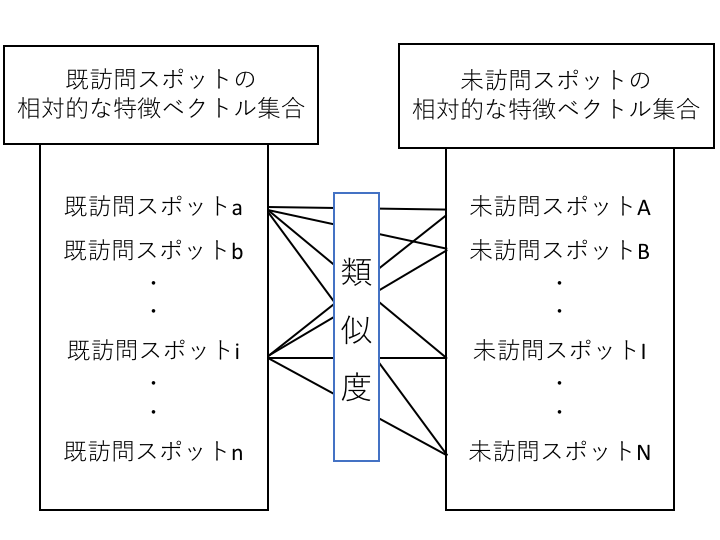
\includegraphics[clip,width=7.0cm]{picture/Photo_CosSim_jap.png}
    \caption{類似度計算概念図}
    \label{fig:photo_cossim}
    \end{center}
\end{figure}

本研究では,観光スポットの特徴は相対的な特徴を利用する.
相対的な特徴とは,特定の観光スポットが,ある観光スポット集合に含まれた他の観光スポットと比較した場合における独特な特徴である.
例として,観光スポット集合内に鹿苑寺と清水寺が存在する場合を考える.
このとき鹿苑寺の特徴は,金色,金箔,輝き等となり,清水寺の特徴は,舞台,胎内,一望等となる.
どちらも京都に存在する寺院であるため,京都や寺院に関連する特徴は独特な特徴として現れることがない.
次に,観光スポット集合内に東京都庁舎展望台と鹿苑寺が存在する場合を考える.
このとき鹿苑寺の特徴は,金閣寺,お寺,金色,京都等となり,東京都庁舎の特徴は,展望,夜景,新宿等となる.
観光スポットのカテゴリが大きく異なる場合であれば,カテゴリとしての特徴が現れる.
また,スポット自身の特徴を表すことができる.
本研究では,あるスポットが集合内の他のスポットと比較するとき,より各スポットの特徴を明らかにできる相対的な特徴に着目して研究を行う.

スポット差分ベクトルは式\ref{math:Vector difference}として定義される.
スポット差分ベクトルを求めるスポットを除いたスポット集合の各スポットのスポットベクトルの平均値を引いた値となる.
$spot_{set} =\{s_1,s_2,\dots,s_i,\dots,s_n\}$は既訪問スポット集合や未訪問スポット集合となっている.
また,$s_i$は集合内のある観光スポットを示している.
\begin{equation}
  v_i=s_i-average(spot_{set}-s_i)
    \label{math:Vector difference}
\end{equation}


%%%%%%%%%%%%%%%%%%%%%%%%%%%%%%%%%%%%%%%%%%
\subsection{説明スポットの決定}
\label{subsec:説明スポットの決定}

既訪問スポットの各特徴差分ベクトル$v_i$と未訪問スポットの各特徴差分ベクトル$v_j$から,既訪問スポットと未訪問スポット間の相対的な特徴の類似度(図\ref{fig:photo_cossim})を求める.
類似度計算には,コサイン尺度(式\ref{math:CosSim})を用いる.
\begin{eqnarray}
cos(v_i,v_j)=\frac{v_{i1}v_{j1}+v_{i2}v_{j2}+\cdots+v_{in}v_{jn}}
{\sqrt{v^2_{i1}+\cdots+v^2_{in}}\times\sqrt{v^2_{j1}+\cdots+v^2_{jn}}}
\label{math:CosSim}
\end{eqnarray}

既訪問スポットの各特徴ベクトルと未訪問エリア内の各特徴ベクトルの類似度が0.125以上かつ,類似度が最も高い既訪問スポットと未訪問スポットの関連付けを行う.
また,既訪問スポットと未訪問スポットとの関連をつけるとき以下の2つの方法がある.

\begin{enumerate}
  \item 既訪問スポットをベースにして未訪問スポットと関連付ける方法
  \item 未訪問スポットをベースにして既訪問スポットと関連付ける方法
\end{enumerate}

方法1では,既訪問スポットをベースにすると未訪問エリア内のスポットが複数の特徴を保持する場合は同じ未訪問スポットと関連づける場合がある.
方法2では,未訪問スポットをベースにすることによって,既訪問スポット集合から各スポットの特徴を取り出し,未訪問スポットと関連付けることができるため,方法2を利用する.
また,本研究では,未訪問スポットを説明するため未訪問スポットをベースにすることが妥当と考えられる.

%%%%%%%%%%%%%%%%%%%%%%%%%%%%%%%%%%%%%%%%%%
\subsection{説明するための役割語の抽出}
\label{subsec:説明するための役割語の抽出}
観光スポットのレビューはすべて形態素解析器「mecab-ipadic-NEologd」を使用することで,単語抽出処理を行う.
しかし,これらを用いて得られた単語は,日本語として成立しない語が含まれており,これらノイズの削除が必要となる.
具体的には,助詞,助動詞,連体詞,記号,ストップワードを削除する(表\ref{table:mecab}).

\begin{table}[t]
  \caption{形態素解析の例}
  \label{table:mecab}
  \centering
    \begin{tabular}{c|p{23zw}} \hline
      レビュー文書 & 園内も広く,気分転換に散歩したりするのにちょうどよい.きれいに清掃などもされていて,気分がよいです.\\
      \hline
      形態素解析 & 園内 広い 気分転換 散歩 ちょうど よい きれい 清掃 さ れ い 気分 よい\\
      \hline
    \end{tabular}
\end{table}

節\ref{subsec:説明スポットの決定}で関連付けした既訪問スポットと未訪問スポットの情報は単語形式でユーザに提示するため,ある観光スポットのレビュー集合を文書$i$とし,$i$に対する単語$j$が出現するスポット集合の出現回数を$TF_{i,j}$,単語$j$がスポット集合の文書数を$DF_{j}$,スポット集合内の全スポット数を$|D|$とした時,そのスポットにおける単語の特徴量は,式\ref{math:TFIDF}で定義される.

\begin{equation}
  word_{i,j} = TF_{i,j} \times IDF_{j}
  \label{math:TFIDF}
\end{equation}
\begin{equation}
  IDF_{j} = log(\frac{|D|}{DF_{j}})
  \label{math:IDF}
\end{equation}

本手法では,既訪問スポットに関して,ユーザが複数個のスポットを入力する.
それぞれのスポットの全レビューをまとめて1つの文書と見なし,それ以外のスポットの全レビューも文書とみなすことで,式\ref{math:TFIDF},\ref{math:IDF}によってTFIDF値を算出し,既訪問スポット毎の特徴語とする.

未訪問エリアに関して,ユーザがエリアを指定して入力する.
エリア内のそれぞれのスポットの全レビューをまとめて1つの文書と見なし,それ以外のスポットの全レビューも文書とみなすことで,式\ref{math:TFIDF},\ref{math:IDF}によってTFIDF値を算出し,未訪問エリアのスポット毎の特徴語とする.

関連付けした既訪問スポットと未訪問スポットの説明情報は,TFIDFで求めた各スポットの特徴語による調和平均を用いて決定する.
調和平均とは,逆数の算術平均の逆数である.
既訪問スポットのレビュー文書と,未訪問スポットのレビュー文書に,共通して出現する単語を抽出する.抽出した単語のスコアは式\ref{math:Harmonic Mean}によって定義する.
$word_{familiar}$と$word_{unfamiliar}$は同じ単語がそれぞれ既訪問スポットのTFIDF値と未訪問スポットのTFIDF値を示している.
単語スコアの値が大きと既訪問スポットと未訪問スポットのそれぞれのTFIDF値が大きい,つまり単語がそれぞれの文書に置いて重要度が高いことを示している.
よって,単語スコアの上位10個の単語を説明情報としてユーザに提示する(図\ref{fig:photo_map}).
\begin{eqnarray}
  score=\frac{1}{\frac{1}{2}(\frac{1}{word_{familiar}}+\frac{1}{word_{unfamiliar}})}
  \label{math:Harmonic Mean}
\end{eqnarray}

\begin{figure}[t]
  \begin{center}
    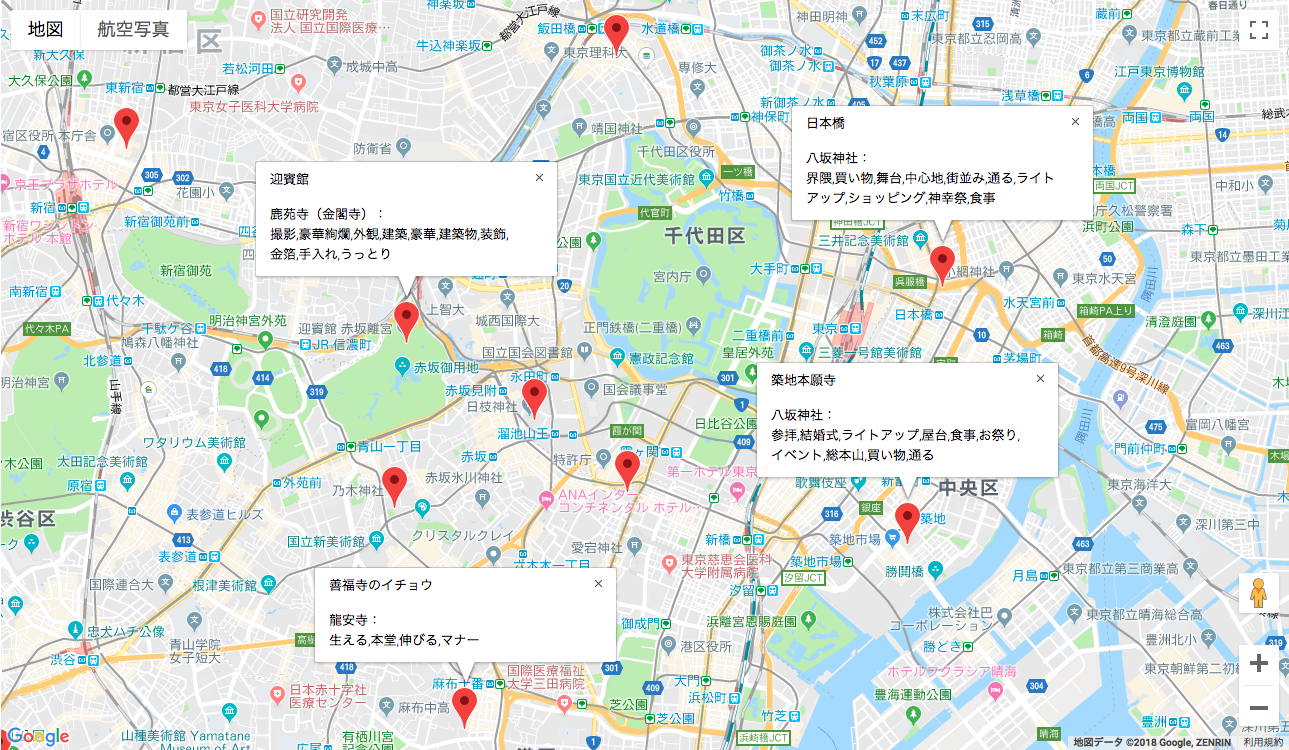
\includegraphics[clip,width=8.0cm]{picture/Photo_Map.png}
    \caption{説明手法インターフェース}
    \label{fig:photo_map}
   \end{center}
\end{figure}

%%%%%%%%%%%%%%%%%%%%%%%%%%%%%%%%%%%%%%%%%%
\subsection{未訪問スポットの説明情報の例}
\label{subsec:未訪問スポットの説明情報の例}
表\ref{table:既訪問スポット集合と未訪問スポット集合}は,ユーザが既に訪問したことがあるスポットと,未訪問スポットの集合の例である.未訪問スポットは東京都内からランダムに選んだ5つのスポットである.
節\ref{sec:未訪問スポットの説明手法}の提案手法を使って説明単語を求めた結果は表\ref{table:説明情報の例}である.

公園という特徴に注目すると,未訪問スポット集合内で最も公園に近いスポットは新宿御苑であると考えられる.
既訪問スポット集合内には小田原城址公園と奈良公園の二つの公園がある.
小田原城址公園には花や遊具に対する記述が多く,奈良公園は鹿や草に対する記述が多い.
新宿御苑は花や遊具に対する記述が多いため,小田原城址公園との関連性があると考えられる.


三島スカイウォークは既訪問スポット集合内で眺めがいい,高いの特徴が1番強いことが考えられる.
未訪問スポット集合内で眺めがいい,高いの特徴が強いのは東京スカイツリーや東京タワー大展望台の2つがある.
東京スカイツリーはより高いによって三島スカイウォークと考えられるが,説明情報を見ると富士山が入っている.
2つスポットの高さは富士山という単語によって強調されている.
提案手法は各集合のスポット毎の特徴を表すことができる.

\begin{table}[t]
  \caption{既訪問スポット集合と未訪問スポット集合}
  \label{table:既訪問スポット集合と未訪問スポット集合}
  \centering
  \begin{tabular}{l|l}
  \hline
  \multicolumn{1}{c|}{既訪問スポット名} & \multicolumn{1}{c}{未訪問スポット名} \\ \hline
  浅草寺                           & 東京ディズニーランド(R)                \\
  小田原城址公園                       & 新宿御苑                         \\
  伏見稲荷大社                        & 東京スカイツリー                     \\
  奈良公園                          & 東京タワー大展望台                    \\
  三島スカイウォーク                     & 明治神宮                         \\ \hline
  \end{tabular}
\end{table}


\begin{table*}[t]
  \caption{説明情報の例}
  \label{table:説明情報の例}
  \centering
  \begin{tabular}{l|l|l}
  \hline
  \multicolumn{1}{c|}{未訪問スポット} & \multicolumn{1}{c|}{既訪問スポット} & \multicolumn{1}{c}{説明情報}                     \\ \hline
  新宿御苑                      & 小田原城址公園                         & お花見,咲き誇る,園内,桜の時,のんびり,手入れ,自然,遊具,ツツジ          \\
  東京スカイツリー                     & 三島スカイウォーク                    & 富士山,揺れ,高所恐怖症,揺れる,天井,絶景,エレベーター,パノラマ,展望デッキ,昇る \\ \hline
  \end{tabular}
\end{table*}


%%%%%%%%%%%%%%%%%%%%%%%%%%%%%%%%%%%%%%%%%%
%%%%%%%%%%%%%%%%%%%%%%%%%%%%%%%%%%%%%%%%%%
\section{評価実験}
\label{sec:評価実験}
%%%%%%%%%%%%%%%%%%%%%%%%%%%%%%%%%%%%%%%%%%
%%%%%%%%%%%%%%%%%%%%%%%%%%%%%%%%%%%%%%%%%%
%%%%%%%%%%%%%%%%%%%%%%%%%%%%%%%%%%%%%%%%%%

\subsection{実験内容}

絶対的な特徴と提案手法の相対的な特徴による説明情報を提示する方法の比較を行う.
また,相対的な特徴を利用する場合において,調和平均を利用して単語スコアを算出する方法と相加平均を利用して単語スコアを算出する方法の比較を行った.

クラウドソーシングのサービスである,CrowdWorks\footnote{https://crowdworks.jp/}を利用して24人の被験者を集めた.
じゃらんで取得した観光スポットを使って,被験者の既訪問スポットの選択による未訪問スポットの説明情報の提示を行った.
絶対的な特徴と相対的な特徴の説明情報のパターンは以下の4つとなる.
\begin{description}
  \item A.絶対的な特徴(カテゴリ,滞在時間,訪問時期)
  \item B.絶対的な特徴(特徴ベクトル)
  \item C.相対的な特徴(差分ベクトル,調和平均を利用して単語スコアを算出)
  \item D.相対的な特徴(差分ベクトル,相加平均を利用して単語スコアを算出)
\end{description}

説明情報Aは,観光スポット検索サイトでスポットを検索するためで使う絞り込み情報である.絞り込み情報は例は以下の3つである.
\begin{itemize}
 \item カテゴリ:神社・神宮・寺院,観光施設・名所巡り等
 \item 滞在時間:1時間未満,1\verb|~|2時間等
 \item 訪問時期:1\verb|~|12月,春,夏,秋,冬
\end{itemize}
まず,既訪問スポットを使って,未訪問スポットとのカテゴリが一致がどうか,滞在時間と一致かどうか,訪問時期と一致かどうかの順で徐々に情報を絞って,既訪問スポットと未訪問スポットの対応付けを行う.
次に,絞った後の未訪問スポットが複数残った場合,レビュー数が1番多い未訪問スポットを利用する.
最後に,節\ref{subsec:説明するための役割語の抽出}を使って説明するための役割語を抽出し,被験者に提示する.
説明情報Bは,節\ref{subsec:スポットのレビューから特徴ベクトル生成}で作成した特徴ベクトルを使って,各スポットの特徴とする.
説明情報Cは,提案手法である.
説明情報Dは,関連付けした既訪問スポットと未訪問スポットの説明情報は,TFIDFで求めた各スポットの特徴語による調和平均を用いて決定する.
既訪問スポットのレビュー文書と,未訪問スポットのレビュー文書に,共通して出現する単語を抽出する.
また,抽出した単語のはぞれぞれのスポットのTFIDFの値の平均を以上である必要がある.
既訪問スポット単語のTFIDF値と未訪問スポット単語のTFIDF値の差の絶対値を単語スコアとして算出し,単語スコアが最も0に近い10個の単語を説明情報として被験者に提示する.

まず,被験者は既に訪問したことがあり,気に入った観光スポットを4つ以上10つ以下入力した.
入力するスポットは,検索候補から選んでもらう.
例えば,新宿御苑---新宿,清水寺---京都などがある.
次に,被験者は旅行等で行ったことがなく,これから行ってみたい都道府県・エリアを入力した.
説明情報のパターンのAからDの順で処理を行って,ユーザに未訪問スポット名,キーワード,既訪問スポット名を提示し,以下の5つの評価から1つを選択した.
\begin{enumerate}
  \item キーワードなし
  \item 2つのスポットにそもそも関係性があるが,キーワードにより関係が明確になった
  \item 2つのスポットの関係にキーワードにより初めて気がついた
  \item 2つのスポットに関係性があるがキーワードは関係性を表していない
  \item 2つのスポットに関係性はない
\end{enumerate}


\subsection{実験結果と考察}
\label{subsec:実験結果}

\begin{table}[t]
  \caption{実験結果のデータ数の統計}
  \label{table:実験結果のデータ数の統計}
  \centering
  \begin{tabular}{c|r|r|r|r|r}
  \hline
  評価 & \multicolumn{1}{c|}{説明情報A} & \multicolumn{1}{c|}{説明情報B} & \multicolumn{1}{c|}{説明情報C} & \multicolumn{1}{c|}{説明情報D} & \multicolumn{1}{c}{合計} \\ \hline
  1  & 0                      & 0                      & 0                      & 4                      & 4                      \\
  2  & 19                     & 44                     & 32                     & 26                     & 121                    \\
  3  & 20                     & 62                     & 53                     & 56                     & 191                    \\
  4  & 1                      & 3                      & 3                      & 3                      & 10                     \\
  5  & 6                      & 21                     & 21                     & 20                     & 68                     \\\hline
  合計 & 46                     & 130                    & 109                    & 109                    & 394                    \\ \hline
  \end{tabular}
\end{table}

表\ref{table:実験結果のデータ数の統計}は評価1から5の説明情報AからDのそれぞれの実験結果のデータの数である.
今回の実験では,使用可能のデータの合計は394件である.
説明情報Aの方が未訪問スポットと関連がある既訪問スポットの数が最も少ない.
説明情報Bの方が未訪問スポットと関連がある既訪問スポットの数が最も多い.
説明情報Cと説明情報Dについて,未訪問スポットと既訪問スポットの関連付け手法は同じであるため,数が同じとなる.

\begin{table}[t]
  \caption{説明情報においての評価の割合}
  \label{table:説明情報においての評価の割合}
  \centering
  \begin{tabular}{c|r|r|r|r}
  \hline
  評価 & \multicolumn{1}{c|}{説明情報A} & \multicolumn{1}{c|}{説明情報B} & \multicolumn{1}{c|}{説明情報C} & \multicolumn{1}{c}{説明情報D} \\ \hline
  1  & 0.00\%                     & 0.00\%                     & 0.00\%                     & 3.67\%                    \\
  2  & 41.30\%                    & 33.85\%                    & 29.36\%                    & 23.85\%                   \\
  3  & 43.48\%                    & 47.69\%                    & 48.62\%                    & 51.38\%                   \\
  4  & 2.17\%                     & 2.31\%                     & 2.75\%                     & 2.75\%                    \\
  5  & 13.04\%                    & 16.15\%                    & 19.27\%                    & 18.35\%                   \\ \hline
  \end{tabular}
\end{table}

表\ref{table:説明情報においての評価の割合}は説明情報AからDにおいて評価1から5の実験結果のデータの数の割合である.
被験者に提示する説明情報Aは,未訪問スポットと既訪問スポットがそもそも関連性があり,またキーワードを提示することによってさらに明確となった.
説明情報Dは,未訪問スポットと既訪問スポットに関連性がないと思っていたが,被験者にキーワードを提示することによって初めて気がついたため,本研究の提案手法に関連性がある.
説明情報Cと説明情報Dは,被験者に提示する未訪問スポットと既訪問スポットがそもそも関連性がない割合が多い.
4つの説明情報パターンにおいて説明情報Dのみ被験者に提示するキーワードがない.
よって,調和平均を利用することによって 被験者にキーワードを提示することができる場合が多いといえる.
また,評価1,評価4と評価5は説明情報を意味がなしていないことが示すことができる.
よって,説明情報Dは最も意味をなしていないことがいえる.

評価1と評価2はから,被験者に提示する未訪問スポットと既訪問スポットがそもそも関連性があるカテゴリを利用する場合が1番良いでる.
しかし,関連性のあるスポットの数はカテゴリに制限しているため被験者に提示できる数も少ない.
また,別カテゴリのスポット情報を被験者に提示できないため意外性を求めることができないといえる.
2番目は特徴ベクトル利用する場合,3番目は差分ベクトルと調和平均の組み合わせるとき,最も良くないのは説明情報Dの差分ベクトルと相加平均の組み合わせである.
説明情報Cと説明情報Dの関連性があるスポットの数が同じであるが,相加平均を使って単語スコアを算出することによって被験者に提示するキーワードの理解支援の役割が減少したといえる.

評価2は差分ベクトルと相加平均の組み合わせが最も良い,差分ベクトルと調和平均の組み合わせが2番目良い,3番目は特徴ベクトル利用する場合,最も良くないのはカテゴリを用いる場合である.
よって,説明情報Bの特徴ベクトルと説明情報Cの差分ベクトルと調和平均の組み合わせが良い結果を示すことができるといえる.
また,差分ベクトルを利用することによって被験者に意外性があり,カテゴリに拘らない未訪問スポットを提示することができる.

\begin{table}[t]
  \caption{既訪問スポットのカテゴリが異なる場合と類似する場合の評価の割合}
  \label{table:既訪問スポットのカテゴリが異なる場合と類似する場合の評価の割合}
  \centering
  \begin{tabular}{c|r|r}
  \hline
  & \multicolumn{1}{c|}{\begin{tabular}[c]{@{}c@{}}既訪問スポットが\\ 異なる場合\end{tabular}} & \multicolumn{1}{c}{\begin{tabular}[c]{@{}c@{}}既訪問スポットが\\ 類似する場合\end{tabular}} \\ \hline
  説明情報B\_評価1 & 56.82\%                            & 43.18\%                            \\
  説明情報C\_評価1 & 71.87\%                            & 28.13\%                            \\ \hline
  説明情報B\_評価2 & 51.61\%                            & 48.39\%                            \\
  説明情報C\_評価2 & 52.83\%                            & 47.170\%                            \\ \hline
\end{tabular}
\end{table}

説明情報Bと説明情報Cについて,被験者が入力した既訪問スポットのカテゴリが異なる場合と類似する場合のとき,評価2と評価3の評価の割合は表\ref{table:既訪問スポットのカテゴリが異なる場合と類似する場合の評価の割合}となる.
提案手法である説明情報Cを使うと,被験者が既に訪問したあるスポットと関係なしで,被験者が有意味のキーワードを提示することができる.
差分ベクトルを利用することによって,カテゴリに渡って各スポットの特徴を求めることができるといえる.
既訪問スポットのジャンルが類似する場合では説明情報Bの方かより良い評価となっている.

% 節\ref{subsec:Presenting similar information by harmonic mean}では,調和平均を利用して単語スコアを算出し,上位10個の単語を説明情報としてユーザに提示するの提案手法について,妥当性を調査する実験を行った.
%
% %%%%%%%%%%%%%%%%%%
% \subsubsection{実験内容}
% % 調和平均を利用して類推情報を提示する場合と,各スポットの平均の重みを利用する場合の比較を行った.まず,訪問スポットのレビュー文書と,未訪問スポットのレビュー文書に,共通して出現する単語を抽出する.次は,閾値を決めて各スポットのTFIDF値の平均以上の単語を抽出する.具体的に,既訪問スポット集合の各スポットのTFIDF値の平均を計算し,スポット毎の単語のTFIDF値が各スポットの平均の重み以上であるかどうか判断する.また,未訪問スポットも同様な算出方法を使っての集合の各スポットのTFIDF値の平均を計算し,スポット毎の単語のTFIDF値が各スポットの平均の重み以上であるかどうか判断する.既訪問スポット単語スコアと未訪問単語スコアの差の絶対値が0に近いと,それぞれのスポットにおいての単語の意味合いが近いと示している.よって,差の絶対値が0に近い10個の単語を類推情報としてユーザに提示
% % する.
% 調和平均を利用して類推情報を提示する場合と,相加平均を利用する場合の比較を行った.まず,訪問スポットのレビュー文書と,未訪問スポットのレビュー文書に,共通して出現する単語を抽出する.次は,
%
% 閾値を決めて各スポットのTFIDF値の平均以上の単語を抽出する.具体的に,既訪問スポット集合の各スポットのTFIDF値の平均を計算し,スポット毎の単語のTFIDF値が各スポットの平均の重み以上であるかどうか判断する.また,未訪問スポットも同様な算出方法を使っての集合の各スポットのTFIDF値の平均を計算し,スポット毎の単語のTFIDF値が各スポットの平均の重み以上であるかどうか判断する.既訪問スポット単語スコアと未訪問単語スコアの差の絶対値が0に近いと,それぞれのスポットにおいての単語の意味合いが近いと示している.よって,差の絶対値が0に近い10個の単語を類推情報としてユーザに提示
% する.
%
% %%%%%%%%%%%%%%%%%%
% \subsubsection{実験結果と考察}
%
%
%
% \subsection{対応付けの比較実験}
% \label{subsec:Comparative experiment of correspondence}
% 節\ref{subsec:Calculation of similarity by cosine similarity}では,既訪問スポット集合と未訪問スポット集合それぞれの各スポットベクトルと他のスポットベクトルを使って類似度を計算することで観光スポットの相対的な特徴を求める手法について,妥当性を調査する予備実験を行なった.
%
% %%%%%%%%%%%%%%%%%%
% \subsubsection{実験内容}
% \label{subsec:FF Experiment Contents}
% 既訪問スポット集合と未訪問スポット集合それぞれの各スポットベクトルと他のスポットベクトルを使って類似度を計算する場合と,節\ref{subsec:Calculation of similarity by cosine similarity}の既訪問スポット集合と未訪問スポット集合それぞれの各スポットベクトルと他のスポットベクトルの差分を使って類似度を計算する場合のスポットの比較を行った.
% 表\ref{table:既訪問スポット集合とみ訪問スポット集合}は,実験で使う既訪問スポット集合と未訪問スポット集合である.既訪問スポット集合は京都の寺院・神社のカテゴリーから5つの観光スポットを選んだ.未訪問スポット集合は東京都に存在する観光スポットから複数のカテゴリーに渡って5つの観光スポットを選んだ.
% \begin{table}[t]
%     \caption{既訪問スポット集合とみ訪問スポット集合}
%     \label{table:既訪問スポット集合とみ訪問スポット集合}
%     \centering
%     \begin{tabular}{|l|l|}
%     \hline
%     \multicolumn{1}{|c|}{既訪問スポット} & \multicolumn{1}{c|}{未訪問スポット} \\ \hline
%     鹿苑寺(金閣寺) & 皇居東御苑    \\ \hline
%     八坂神社  & 新宿御苑   \\ \hline
%     清水寺   & 東京都庁舎展望室        \\ \hline
%     龍安寺   & 浅草寺      \\ \hline
%     伏見稲荷大社   & 明治神宮       \\ \hline
%     \end{tabular}
% \end{table}
%
% %%%%%%%%%%%%%%%%%%
% \subsubsection{実験結果と考察}
% \label{subsec:FF Results AND Discussion}
% \begin{table}[t]
%     \caption{特徴ベクトルや特徴差分ベクトルを利用する時の実験結果}
%     \label{table:特徴ベクトルや特徴差分ベクトルを利用する時の結果}
%     \centering
%     \begin{tabular}{|l|l|l|l|}
%     \hline
%     \multicolumn{2}{|c|}{特徴ベクトルを利用}  & \multicolumn{2}{c|}{特徴差分ベクトルを利用} \\ \hline
%     \multicolumn{1}{|c|}{\begin{tabular}[c]{@{}c@{}}既訪問\\\end{tabular}} &
%     \multicolumn{1}{c|}{\begin{tabular}[c]{@{}c@{}}類似未訪問\\スポット\end{tabular}} &  \multicolumn{1}{c|}{\begin{tabular}[c]{@{}c@{}}既訪問\\\end{tabular}} & \multicolumn{1}{c|}{\begin{tabular}[c]{@{}c@{}}類似未訪問\\スポット\end{tabular}} \\ \hline
%     鹿苑寺&明治神宮&鹿苑寺&新宿御苑   \\ \hline
%     八坂神社&明治神宮&八坂神社&明治神宮   \\ \hline
%     清水寺&浅草寺&清水寺&浅草寺   \\ \hline
%     龍安寺&明治神宮&龍安寺&皇居東御苑  \\ \hline
%     伏見稲荷大社&明治神宮&伏見稲荷大社&明治神宮   \\ \hline
%     \end{tabular}
% \end{table}
% 表\ref{table:特徴ベクトルや特徴差分ベクトルを利用する時の結果}は実験結果となっている.特徴ベクトルを利用する場合,既訪問スポットのカテゴリーは寺院・神社であるため,類似する未訪問スポットもカテゴリーによって影響される.未訪問スポットの5つのスポットからカテゴリーが一致するスポットが類似スポットになる結果になている.
%
% 一方,節\ref{subsec:Calculation of similarity by cosine similarity}の提案手法を利用する場合,既訪問スポット集合内の鹿苑寺や龍安寺と他のスポットと比較するとき庭園という相対的な特徴を見つけることができる.同様に,未訪問スポット集合内の新宿御苑や皇居東御苑と他のスポットと比較するとき庭園という相対的な特徴を見つけることができる.結果,鹿苑寺と新宿御苑,龍安寺と皇居東御苑を関連づけることができる.また,鹿苑寺の庭園特徴に関して,同じく庭園特徴の新宿御苑と関連ずける理由として鹿苑寺は庭園中に金閣が建ているに対して,新宿御苑は庭園中に旧御凉亭が建ていることから,庭園以外の要素も考量して類似性を求めていることがわかった.よって,既訪問スポット集合と未訪問スポット集合それぞれの各スポットベクトルと他のスポット差分ベクトルの方はより観光スポットの相対的な特徴を求めることができる.


%%%%%%%%%%%%%%%%%%%%%%%%%%%%%%%%%%%%%%%%%%
\section{まとめと今後の課題}
\label{sec:まとめと今後の課題}
%%%%%%%%%%%%%%%%%%%%%%%%%%%%%%%%%%%%%%%%%%
本研究では,ユーザが行きたい観光スポットが決まっていない場合,ランキング,おすすめ情報やカテゴリなどに観光検索情報を使用することによって,検索した観光スポットがに対する理解が困難であることを着目した.
未訪問スポットに対する理解を支援するために,ユーザが既に訪問したことがあるスポットの特徴を未訪問スポットにあてはめて理解を支援する説明手法を提案した.

評価実験では4つの説明情報パターンを用いて比較を行った.
結果,カテゴリを利用する場合では,未訪問スポットと関連する既訪問スポットが最も少ない.
差分ベクトルと相加平均を利用する場合では,キーワードの理解を支援する役割が最も少ない.
差分ベクトルと調和平均を利用することによって,各スポットの特徴を求めることができる.
また,意外性がある未訪問スポットと既訪問スポットを関連付けることができ,ユーザが知らない観光スポットに対する興味と関心を引き出すことができる可能性があることを確認した.

今後の課題としては,実験時に得られたユーザに提示するキーワード,未訪問スポットと既訪問スポットのカテゴリの関連性を分析する.
また,ユーザに提示する各キーワードの有効性と関連性についての評価を行う予定である.

% 今後の課題としては,関東圏内の観光スポットを使っているため,有名でない観光スポットは東京都以外の県に集中している.次回では,範囲を東京都内に変更して,都内の有名でないかつユーザに満足する観光スポットを検索できるかについて調査する.ユーザが観光スポットを検索するために,レビュー選択する時に新たな分析方法があげられる.今回の実験では,選択したレビューを分析する時,形態素解析を使っているため,レビューは単語に分けられ,単語に重み付けを行うことに対して,ユーザは句のキーワードを選択している場合がある.結果,検索された観光スポットは選択したレビューの中で重みの高い単語を重要視した観光スポットになる.今後,レビューを分析する時に新たな重み付けの方法を検討する必要がある.また,実験時に得られたユーザの観光スポットに対する要求の詳細な分析,要求の判断基準の設定とその妥当性についての評価を行う予定である.

%%%%%%%%%%%%%%%%%%%%%%%%%%%%%%%%%%%%%%%%%%
\section*{謝辞}
%%%%%%%%%%%%%%%%%%%%%%%%%%%%%%%%%%%%%%%%%%
% 本研究の一部は,平成29年度科研費若手研究(B)(課題番号:15K16091),および挑戦的萌芽研究(課題番号:16K12536)によるものです.ここに記して謝意を表すものとします.


%%%%%%%%%%%%%%%%%%%%%%%%%%%%%%%%%%%%%%%%%%
% 文献 Reference
%%%%%%%%%%%%%%%%%%%%%%%%%%%%%%%%%%%%%%%%%%
%\vspace{30mm} <- 文献が本文と近すぎるときは適宜利用してください.
\vspace{2em}
\begin{thebibliography}{99}
% \bibitem{Codd01}
%   廣嶋 伸章,安田 宜仁,藤田 尚樹,片岡 良治,
%     地理情報検索におけるクエリ入力支援のための特徴語の提示,
%     第26回人工知能学会全国大会, Vol.26, 1C1-R-5-6, 2012
% \bibitem{Codd02}
%   松本 敦志,杉本 徹,
%     クチコミから抽出した特徴語を利用する観光地検索支援,
%     第75回全国大会講演論文集, Vol.2013, No.1, pp.307-308, 2013
% \bibitem{Codd03}
%   上原 尚,嶋田 和孝,遠藤 勉,
%     Web上に混在する観光情報を活用した観光地推薦システム,
%     社団法人 電子情報通信学会,信学技報, Vol.112, No.367, pp.13-18, 2012
% \bibitem{Codd04}
%   野守 耕爾,神津 友武,
%     口コミデータにPLSAを適用した観光客目線による観光地分析,
%     第29回人工知能学会全国大会, Vol.29, 1J2-OS-18a-2, pp.1-4, 2015
% \bibitem{Codd05}
%   Gick, M.L. and Holyoak, K.J.:
%   Analogical Problem Solving,
%   Cognitive Psychology, Vol.12, pp.306–355, 1980
% \bibitem{Codd06}
%   石田 純太,砂山 渡,
%     新知識を理解するための類推能力の育成,
%     第30回人工知能学会全国大会, Vol.30, 3F3-3, 2016
% \bibitem{Codd07}
%   砂山 渡, 石田 純太,川本 佳代,西原 陽子,
%     類推による説明スキルの獲得支援システム,
%     情報処理学会論文誌, Vol.59, No.10, 1922–1931, 2018
% \bibitem{Codd08}
%   中村 潤,大澤 幸生,
%     概念創造のための類推思考プロセスにおける迷いの効果,
%     横幹, Vol.2, No.1, p.40-48, 2008
% \bibitem{Codd09}
%   Gentner, D.: Structure-Mapping:
%   A Theoretical Framework for Analogy,
%   Cognitive Science, Vol.7, pp.155–170, 1983
\bibitem{Codd01}
  K. J. Holyoak and P. Thagard,
    ``Mental Leaps: Analogy in Creative Thought, MIT Press'',
    % Cambridge, 1995 %英語用
    Journal of Japanese Society for Artificial Intelligence,  Vol.11, No.3,  pp.489, 1996
\bibitem{Codd02}
  D. Gentner,
    ``Structure-Mapping: A Theoretical Framework for Analogy'',
    Cognitive Science, Vol.7, pp.155–170, 1983
\bibitem{Codd03}
  M. L. Gick and K. J. Holyoak,
    ``Analogical Problem Solving'',
    Cognitive Psychology, Vol.12, pp.306–355, 1980
\bibitem{Codd04}
  M. L. Gick and K. J. Holyoak,
    ``Scheme Induction and Similarity in Analogical Transfer'',
    Cognitive Psychology, Vol.15, pp.1–38, 1983
\bibitem{Codd05}
  Z. Chen and M. W. Daehler,
    ``Positive and Negative Transfer in Analogical Problem-solving by 6-years-old Children'',
    Cognitive Development, Vol.4, No.4, pp.327–344, 1989
\bibitem{Codd06}
  K. J. Holyoak and P. Thagard,
    ``Analogical Mapping by Constraint Satisfaction'',
    Cognitive Science, Vol.13, pp.295–355, 1989
\bibitem{Codd07}
  T. Kurashima, T. Iwata, G. Irie and K. Fujimura.,
    ``Travel route recommendation using geotags in photo sharing sites'',
    CIKM '10 Proceedings of the 19th ACM international conference on Information and knowledge management, pp.579-588, 2010
\bibitem{Codd08}
  R. Kitamura and T. Itoh,
    ``Tourist Spot Recommmendation Applying Generic Object Recognition with Travel Photos'',
    ITE Tech. Rep., Vol.42, No.12, AIT2018-94, pp.185-188, 2018
\bibitem{Codd09}
  A. J. Cheng, Y. Y. Chen, Y. T. Huang and Winston H. Hsu,
    ``Personalized Travel Recommendation by Mining People Attributes from Community-Contributed Photos'',
    MM '11 Proceedings of the 19th ACM international conference on Multimedia, pp.83-92, 2011
\bibitem{Codd10}
  % 日本の形態素解析に条件付きランダムフィールドを適用する
  T. Kudo, K. Yamamoto and Y. Matsumoto,
  ``Applying Conditional Random Fields to Japanese Morphological Analysis'',
  Proceedings of the 2004 Conference on Empirical Methods in Natural Language Processing (EMNLP-2004), pp.230-237, 2004
\end{thebibliography}

\end{document}
